\documentclass[11pt]{amsbook}
\usepackage{../HBSuerDemir}%——————

\begin{document}
%——————
\hPage{b1p1/108}
%——————
\begin{enumerate}
\item[156.]
Sketch the graphs of the relations:
\begin{hEnumerateAlpha}
	\item
	\{(x,y): [x][v] = 1\}
	\item 
	\{(x,y): [x][v] = -1\}
	\item
	\{(x,y): [x][v] = 0\}
	\item
	\{(x,v): [x][v] = 4\}
\end{hEnumerateAlpha}
\item[157.]
Prove

\begin{tabular}{ll}
 a)$[x]\leq x<[x]+1$
 &b)$(a)\leftrightarrow 0\leq x-[x]<1$\\
 c)$[x]+[-x]\leq0$ 
 &d)$0\leq[x]-2[\frac{x}{2}]\leq1$
\end{tabular}
\item[158.]
Given in the figure a window with constant area S.The glass in rectangular form permits the light half of that of semicircular form.Find the amount of light $ \ell(x)\ $ passing through the window.(Glass in rectangular form permits amount of light $ \ell_0\ $ per unit area).
\begin{figure}[htb]
\begin{center}
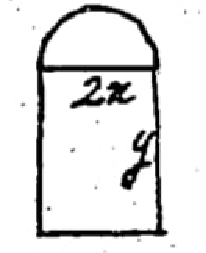
\includegraphics[width=0.20\textwidth]{images/b1p1-108-fig01}
\end{center}
\end{figure}
\item[159.]
Find the area A of an isocales triangle with equal sides a and angle between them is x; then discuss the continuity of A as a function of x.Find m and M.
\item[160.]
Find the distance function d(m) of the foot of the perpendicular from (4,0) to the line y=mx.Find the domain D and range of this functions.
\item[161.]
A variable point P on $ (x - 2)^2 + y^2 = 4 $ is given.Find the sum of the coordinates of P with respect to the line y = x, and y = -x.
\item[162.]
If f($\sqrt{2x}$ + 3) = $x^2$ + x, find f(x).
\item[163.]
If f(x) = $\sqrt{x^2 + 1}$, g(x) = x/($ x^2 $ + 1),find 

\begin{tabular}{ll}
 a)$(fog)(x) $
 &b)$(gof)(x) $\\
 c)$f^-1(x)$
 &d)$g^-1(x) $
\end{tabular}
\end{enumerate}
\end{document}